\documentclass{article}\usepackage{graphicx, color}
%% maxwidth is the original width if it is less than linewidth
%% otherwise use linewidth (to make sure the graphics do not exceed the margin)
\makeatletter
\def\maxwidth{ %
  \ifdim\Gin@nat@width>\linewidth
    \linewidth
  \else
    \Gin@nat@width
  \fi
}
\makeatother

\definecolor{fgcolor}{rgb}{0.2, 0.2, 0.2}
\newcommand{\hlnumber}[1]{\textcolor[rgb]{0,0,0}{#1}}%
\newcommand{\hlfunctioncall}[1]{\textcolor[rgb]{0.501960784313725,0,0.329411764705882}{\textbf{#1}}}%
\newcommand{\hlstring}[1]{\textcolor[rgb]{0.6,0.6,1}{#1}}%
\newcommand{\hlkeyword}[1]{\textcolor[rgb]{0,0,0}{\textbf{#1}}}%
\newcommand{\hlargument}[1]{\textcolor[rgb]{0.690196078431373,0.250980392156863,0.0196078431372549}{#1}}%
\newcommand{\hlcomment}[1]{\textcolor[rgb]{0.180392156862745,0.6,0.341176470588235}{#1}}%
\newcommand{\hlroxygencomment}[1]{\textcolor[rgb]{0.43921568627451,0.47843137254902,0.701960784313725}{#1}}%
\newcommand{\hlformalargs}[1]{\textcolor[rgb]{0.690196078431373,0.250980392156863,0.0196078431372549}{#1}}%
\newcommand{\hleqformalargs}[1]{\textcolor[rgb]{0.690196078431373,0.250980392156863,0.0196078431372549}{#1}}%
\newcommand{\hlassignement}[1]{\textcolor[rgb]{0,0,0}{\textbf{#1}}}%
\newcommand{\hlpackage}[1]{\textcolor[rgb]{0.588235294117647,0.709803921568627,0.145098039215686}{#1}}%
\newcommand{\hlslot}[1]{\textit{#1}}%
\newcommand{\hlsymbol}[1]{\textcolor[rgb]{0,0,0}{#1}}%
\newcommand{\hlprompt}[1]{\textcolor[rgb]{0.2,0.2,0.2}{#1}}%

\usepackage{framed}
\makeatletter
\newenvironment{kframe}{%
 \def\at@end@of@kframe{}%
 \ifinner\ifhmode%
  \def\at@end@of@kframe{\end{minipage}}%
  \begin{minipage}{\columnwidth}%
 \fi\fi%
 \def\FrameCommand##1{\hskip\@totalleftmargin \hskip-\fboxsep
 \colorbox{shadecolor}{##1}\hskip-\fboxsep
     % There is no \\@totalrightmargin, so:
     \hskip-\linewidth \hskip-\@totalleftmargin \hskip\columnwidth}%
 \MakeFramed {\advance\hsize-\width
   \@totalleftmargin\z@ \linewidth\hsize
   \@setminipage}}%
 {\par\unskip\endMakeFramed%
 \at@end@of@kframe}
\makeatother

\definecolor{shadecolor}{rgb}{.97, .97, .97}
\definecolor{messagecolor}{rgb}{0, 0, 0}
\definecolor{warningcolor}{rgb}{1, 0, 1}
\definecolor{errorcolor}{rgb}{1, 0, 0}
\newenvironment{knitrout}{}{} % an empty environment to be redefined in TeX

\usepackage{alltt}
\usepackage[margin=1.25in]{geometry}
\usepackage{graphicx, hyperref, float, multicol, pdflscape, enumerate, paralist}
\usepackage{amssymb,amsmath,amsthm} 
\usepackage[backend=bibtex, natbib=true]{biblatex}
\addbibresource{../references/references.bib}

\usepackage{color}
\newcommand{\ak}[1]{{\color{magenta} #1}}
\newcommand{\mj}[1]{{\color{blue} #1}}

\theoremstyle{plain}
\newtheorem{res}{Result}

\setlength{\parindent}{0cm}
\renewcommand{\baselinestretch}{1.5}

\title{Independence of Periodogram Ordinates at the Fourier Frequencies}
\author{Andee Kaplan \& Maggie Johnson}
\IfFileExists{upquote.sty}{\usepackage{upquote}}{}

\begin{document}

\maketitle



\section{Motivation}

To explore whether it is reasonable to estimate the spectral density of a stationary time series using Bayesian methods. To do this, it is necessary to rely on the asymptotic distributional properties of periodogram ordinates. The motivation behind this work is the following model.
\begin{align}
\label{eq:eqn1}
I_n(\omega_r) |f(\omega_r) &\stackrel{\cdot}{\sim}\text{ indep } \text{Exp}(2\pi f(\omega_r)) \\
\label{eq:eqn2}
f(\omega_r) & \sim \pi(\theta)\\
\label{eq:eqn3}
f(\omega_r) | I_n(\omega_r) &\propto 2\pi f(\omega_r) e^{-2\pi f(\omega_r) y} \pi(\theta)
\end{align}
The periodogram values at $\omega_r$ are only asymptotically distributed as independent exponentials, so to construct the Bayesian model it is essential that the asymptotic behavior in Equation \ref{eq:eqn1} holds. This research uses simulations to assess two results by Lahiri, which state conditions necessary for periodogram ordinates to be asymptotically independent \cite{lahiri2003necessary}.


\section{Background and Problem Statement}

Spectral analysis, or ``frequency domain analysis" is the analysis of stationary time series $\{X_t\}$ by decomposing $\{X_t\}$ into sinusoidal componenets. Spectral analysis is equivalent to ``time domain" analysis based on the autocovariance function, but \mj{can be more useful in certain situations}. The spectral density of a mean-zero stationary process $\{X_t\}$ is used to describe the frequency decomposition of the autocovariance function $\gamma(\cdot)$ and the process $\{X_t\}$. It is the function $f(\cdot)$ defined by 
\begin{align}
f(\lambda) = \frac{1}{2\pi} \sum_{h=-\infty}^{\infty} e^{-ih\lambda} \gamma(h), \hspace{.5cm} -\infty < \lambda < \infty
\end{align}
where $e^{i\lambda}=cos(\lambda)+isin(\lambda)$ and $i=sqrt(-1)$ \cite{brockwell2002introduction}. The periodogram, $I_n(\cdot)$ of $\{X_t\}$ can be regarded as a \mj{sample analogue} of $2\pi f(\cdot)$ \cite{brockwell2002introduction}. The periodogram of $\{x_1,...,x_n\}$ is the function
\begin{align}
I_n(\lambda) = \frac{1}{n} \left\lvert \sum_{t=1}^n x_t e^{-it\lambda} \right\rvert^2
\end{align}

\begin{res} \label{res:first}
Let $f(\omega_r) \not= 0, 1 \le r \le k$ where $f$ denotes the spectral density of a stationary time series $\{X_t\}$. Then when $n\rightarrow \infty$ the joint distribution of the periodogram at $\omega_r$, $I_n(\omega_r)$, tends to that of $k$ mutually indepependent random variables distributed as $\text{Exponential}(2\pi f(\omega_r))$ for $0<\omega_r<\pi$ \cite{brockwell2002introduction}. 
\end{res}

Result~\ref{res:first} describes the asymptotic distribution of a periodogram at fixed frequencies. In practice, this result has often been used with the Fourier frequencies in place of fixed frequencies \mj{reference this} $\{2\pi j/n : j=1,...,n\}$. However, it has been shown that the asymptotic behavior of the periodogram at the Fourier frequencies does not hold as $n \rightarrow \infty$ \mj{(dig into reference to flesh this out)}. Lahiri \cite{lahiri2003necessary} derived two results that describe behavior required for a set of frequencies to satisfy Result~\ref{res:first}

\begin{res} \label{res:lahiri}
In the absense of data tapering,
\begin{enumerate}[(a)]
\item the periodogram values at asymptotically distant ordinates ($I_n(\omega_r)$) are asymptotically independent.  Asymptotically distant ordinates $\{\omega_{ln}\}, \{\omega_{kn}\}$ satisfy $|n(\omega_{ln} - \omega_{kn})| \rightarrow \infty$ as $n \rightarrow \infty$.

\item the periodogram values at asymptotically close ordinates which are asymptotically distant from the sequence $\{0\}$ are asymptotically independent. Asymptotically close ordinates $\{\omega_{ln}\}, \{\omega_{kn}\}$ satisfy $|n(\omega_{ln} - \omega_{kn})| \rightarrow 2\pi l$ for some nonzero integer $l$ as $n \rightarrow \infty$ \cite{lahiri2003necessary}.
\end{enumerate}
\end{res}

%Result~\ref{res:first} gives us the asymptotic distribution of a periodogram at fixed frequencies, while result~\ref{res:lahiri} details properties of frequencies that define where the independence holds. 

Result~\ref{res:lahiri} lends to the idea that a subset of sufficiently spaced and and distant from 0 \texttt{Fourier} frequencies can be constructed such that the periodogram ordinates at these frequencies should be asymptotically independent. \mj{We explore these two results to determine if}, for large $n$,
\begin{enumerate}
  \item Result~\ref{res:first} will not hold at the Fourier frequencies, and
  \item if (1) is true, a subset of Fourier frequencies that are sufficiently spaced and far from 0 can be constructed such that Result~\ref{res:first} holds.
\end{enumerate}

%at at what point distant from zero and at what spacings close to zero do the approximate independence and exponential distribution fail in the periodogram values. 



\section{Models}\label{sec:models}

To explore the asymptotic behavior of the periodogram at the Fourier frequencies, we used several time series models with known spectral densities. The included models are \begin{inparaenum}[\itshape a\upshape)]
\item IID Gaussian(0, 1);
\item AR(1) with $\phi = 0.5$; 
\item AR(4) with $\boldsymbol{\phi} = [0.08, 0.33, 0.1, 0.45$];
\item MA(1) with $\theta = 0.7$;
\item MA(2) with $\boldsymbol{\theta} = [0.7, 0.3$];
\item ARMA(4,1) with $\boldsymbol{\phi} = [0.08, 0.33, 0.1, 0.45$] and $\theta = 0.7$; and
\item ARMA(4,2) with $\boldsymbol{\phi} = [0.08, 0.33, 0.1, 0.45$] and $\boldsymbol{\theta} = [0.7, 0.3$].
\end{inparaenum}

\subsubsection*{IID Gaussian}
The following result about the IID Gaussian model gives us knowledge of the exact, rather than asymptotic, behavior of the periodogram at any frequency.

\begin{res}
For $\{X_t\} \stackrel{\text{IID}}{\sim} \text{N}(0,\sigma^2)$, the periodogram values $\left\{ I_n(\omega_j): \omega_j \in \mathcal{F}_n, \omega_j \not\in \{0,\pi\} \right\}$ are IID Exponential($\sigma^2$) random variables \cite{brockwell2002introduction}.
\end{res}

This model was used as an initial baseline check to support our testing procedure of independent exponentially distributed ordinates. If our procedure showed failure with the IID Gaussian white noise model, then this would be an indication of an issue with the procedure, rather than the frequency spacings. The spectral density of the IID Gaussian model is $f_x(\omega) = \sigma^2/2\pi, \omega \in [-\pi, \pi]$.

\subsubsection*{ARMA(p,q)}
We exclusively used ARMA models as our experimental models because the spectral density of an ARMA model has a known and closed form. An ARMA model is a process $\{X_t\}$ with the form $\phi(B)X_t = \theta(B)Z_t$ where $B$ is the backshift operator and $\{Z_t\}$ is WN(0,$\sigma^2$). Models of this form have spectral density
\begin{align}
f_X(\omega) = \frac{\sigma^2}{2\pi} \frac{|\theta(e^{-i \omega})|^2}{|\phi(e^{-i \omega})|^2}, \omega \in [-\pi, \pi] \text{\cite{brockwell2002introduction}}.
\end{align}

Without the exact knowledge of the spectral density function, we would not be able to test the distributions of the periodogram at each fequencies. \mj{mention moving window?}


\section{Methods}


For Result\ref{res:first} to hold for a known spectral density at the full Fourier frequencies, or a subset of Fourier frequencies $\boldsymbol{\omega}$, the joint asymptotic distribution of the periodogram ordinates $I_n(\omega)$ must be equivalent to the product of n independent exponential distributions with means equal to $2\pi f(\omega)$. It is difficult to test the distribution of the full asymptotic joint distribution, so we split the problem in to two parts: one, a test of asymptotic exponential distribution at each $\omega_i$, and two, a method to test independence over $\omega$. Independence is tested pairwise across all frequencies of interest. We implement the following testing procedure and repeat $s$ simulations of the tests to determine if the tests reject exponentiality and indepence at similar rates as the Type-I errors of our tests ($\alpha$).
\paragraph{Procedure}
\begin{enumerate}
\item Simulate $M$ draws from $X_1,\dots, X_n$ where $\{X_t\}$ is a stationary time series from one of three models.
\item \label{perio}Obtain $M$ periodograms using the fourier frequencies from $(0, \pi)$, $\omega_j = \frac{2\pi j}{n}: j = 1, \dots, \lfloor n/2 \rfloor$.
\item Obtain $\lfloor\frac{n-1}{2}\rfloor$ values of the spectral density at each fourier frequency $f(\omega_j)$. These will be known by design.
\item Simulate $M$ draws from the $\lfloor\frac{n-1}{2}\rfloor$ different distributions $\text{Exp}(2\pi f(\omega_r))$
\item \label{test:exp}Test the distribution of the $M$ values of periodograms at each fourier frequency separately. Store the number of failed tests at each frequency.
\item \label{test:indep}Test the pairwise independence of each neighboring $M$ values of periodograms at each fourier frequency. Store the number of failed tests at each frequency.
\item Inspect the results from steps~\ref{test:exp} and \ref{test:indep} to determine if different spacings of frequencies are needed. If so, use sparcer frequencies and repeat from step~\ref{perio} at the chosen frequencies rather than fourier frequencies.
\end{enumerate}


\subsection{Tests}



\paragraph{Spearman's Rank Correlation}
Spearman's rank correlation $\rho$, is a measure of correlation between a bivariate random sample of size $n$. The calculation of this statistic corresponds to Pearson's $r$ computed on the ranks (and average ranks in the case of ties) of the data. It is used as a test statistic to test the null hypothesis $H_0: \text{ The bivariate random sample } X_i \text{ and } Y_i \text{are mutually independent}$ against the alternative hypothesis $H_1:$ Either there is a tendency for the larger values of $X$ to be paired with the larger values of $Y$ or there is a tendency for the smaller values of $X$ to be paired with the larger values of $Y$. An asymptotic $t$ distribution is used to calculate p-values \cite{conover1998practical}.

We used a two-sided Spearman's rank correlation test at the $\alpha = 0.05$-level to test whether periodogram values at neighboring frequencies (with different inbetween spacings) $\omega_j$ and $\omega_k$ were pairwise independent.


\paragraph{Kolmogorov-Smirnov Test of Distribution}
The Kolmogorov-Smirnov (KS) test is a procedure that uses the maximum vertical distance between an empirical cumulative distribution function and a named cumulative distribution function as a measure of how much the two functions resemble each other. The only assumption of this test is that the data are a random sample. The KS test uses test statistic $T = \sup\limits_x |F^*(x) - S(x)|$ to test the null hypothesis $H_0: F(x) = F^*(x)$ for all $x$, where $F^*(x)$ is the completely specified hypothesized distribution function, $F(x)$ is the unknown distribution function of the data, and $S(x)$ is the empirical distribution function of the data. For data of length $n \le 100$, an exact p-values are available and for data of length $n > 100$, an asymptotic approximation is used \cite{conover1998practical}. The asymptotic distribution is called the Kolmogorov distribution, and is of the form $P(T \le \lambda) = \sum_{k=-\infty}^\infty (-1)^k e^{-2k^2 \lambda^2}$ \cite{kolmogorov1992empirical}.

We used a two-sided KS test at the $\alpha = 0.05$-level to test whether the distributions of our periodogram values at each frequency $\omega_j$ were exponentially distributed with mean parameter $2\pi f(\omega_j)$, where $f(\omega_j)$ is the spectral density evaluated at $\omega_j$.




\section{Results}




\subsection{Tests for Full Fourier Decomposition}

We simulated data, periodograms, and spectral densities for each of the five models discussed in Section~\ref{sec:models} using $M=1000, n=500, s=200$ and $\sigma^2=1$. Tests of asymptotic exponential distribution and pairwise independence were conducted first using the entire set of Fourier frequencies, $\{w_j = \frac{2\pi j}{n}, j=1,...,249\}$ for each of the five models.

\subsubsection{IID Gaussian}
The IID Gaussian white noise model should have periodogram ordinates $I_n(\omega)$ distributed as exactly independent exponentials, regardless of the length of the time series. Figure~\ref{fig:inital-iid} shows the estimated periodogram for one simulated IID Gaussian time series, as well as the constant spectral density. The independence in the time series is clearly seen in the randomness of the periodogram.
\begin{knitrout}
\definecolor{shadecolor}{rgb}{0.969, 0.969, 0.969}\color{fgcolor}\begin{figure}[H]

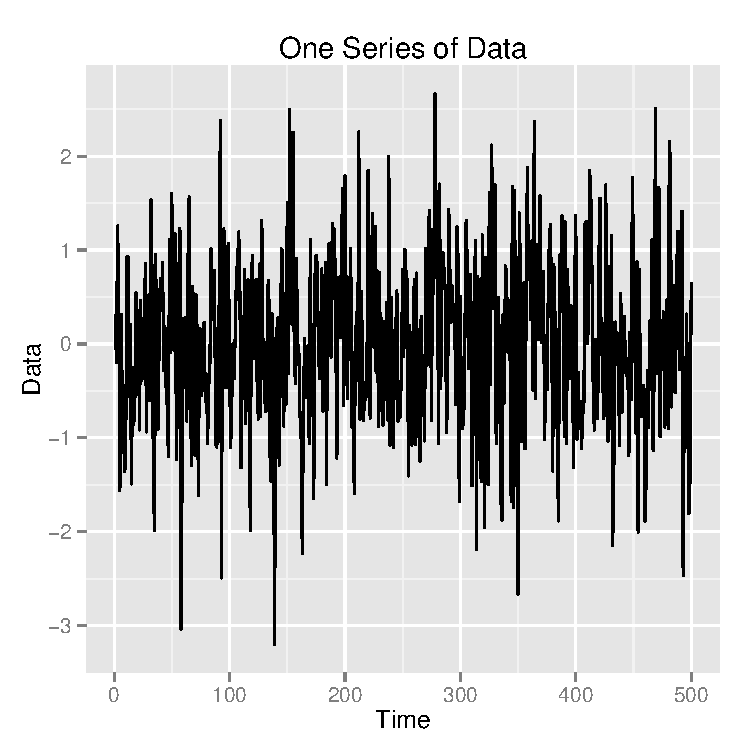
\includegraphics[width=.33\textwidth]{figure/inital-iid1} 
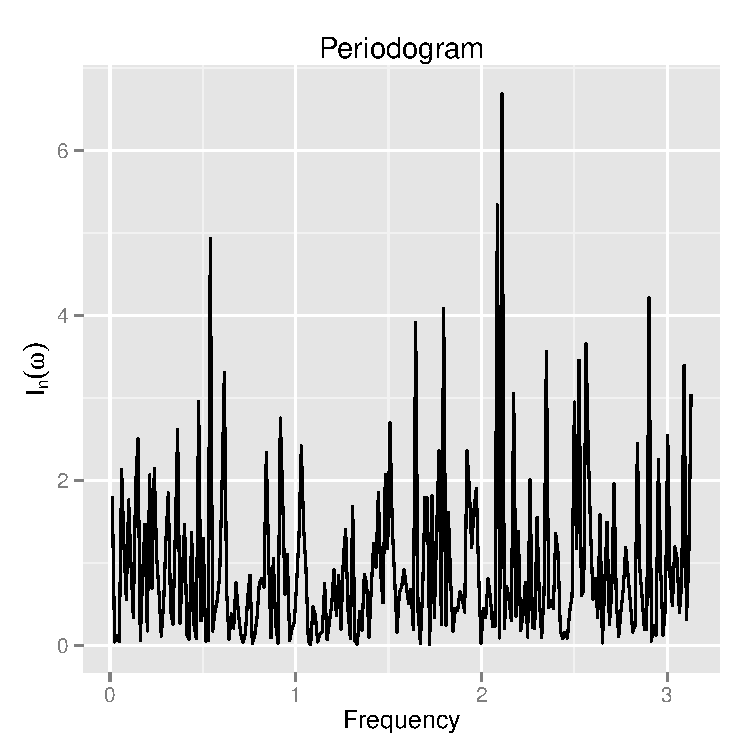
\includegraphics[width=.33\textwidth]{figure/inital-iid2} 
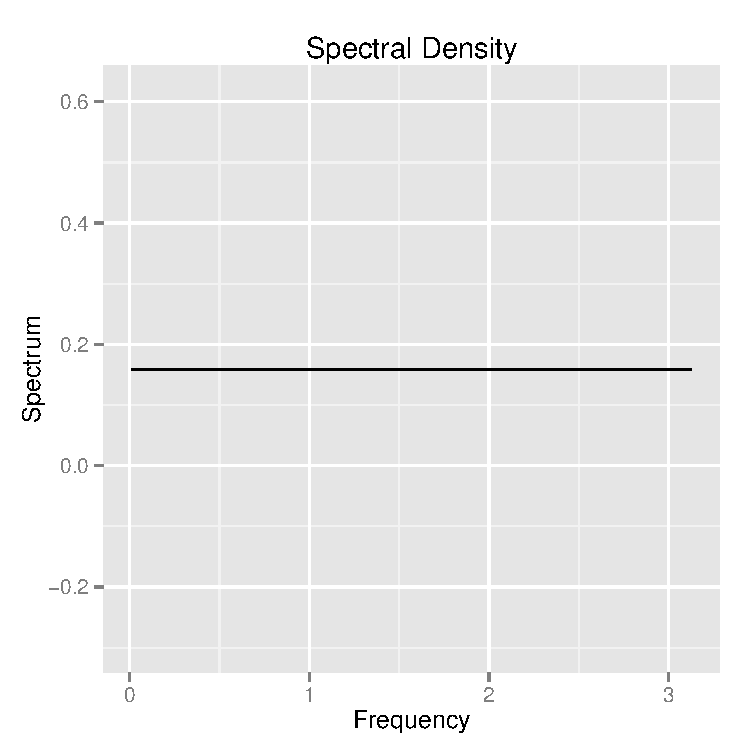
\includegraphics[width=.33\textwidth]{figure/inital-iid3} \caption[One draw, periodogram, and spectral density of a Gaussian IID Model]{One draw, periodogram, and spectral density of a Gaussian IID Model.\label{fig:inital-iid}}
\end{figure}


\end{knitrout}


Tests of exponential distribution and pairwise independence of neighboring Fourier frequencies gave rejection rates relatively similar to the $\alpha$-level of 0.05 over 200 simulations, shown in Figure~\ref{fig:tests-iid}. This suggested that the IID Gaussian model results in independent exponentially distributed periodogram ordinates, as expected.

\begin{knitrout}
\definecolor{shadecolor}{rgb}{0.969, 0.969, 0.969}\color{fgcolor}\begin{figure}[H]

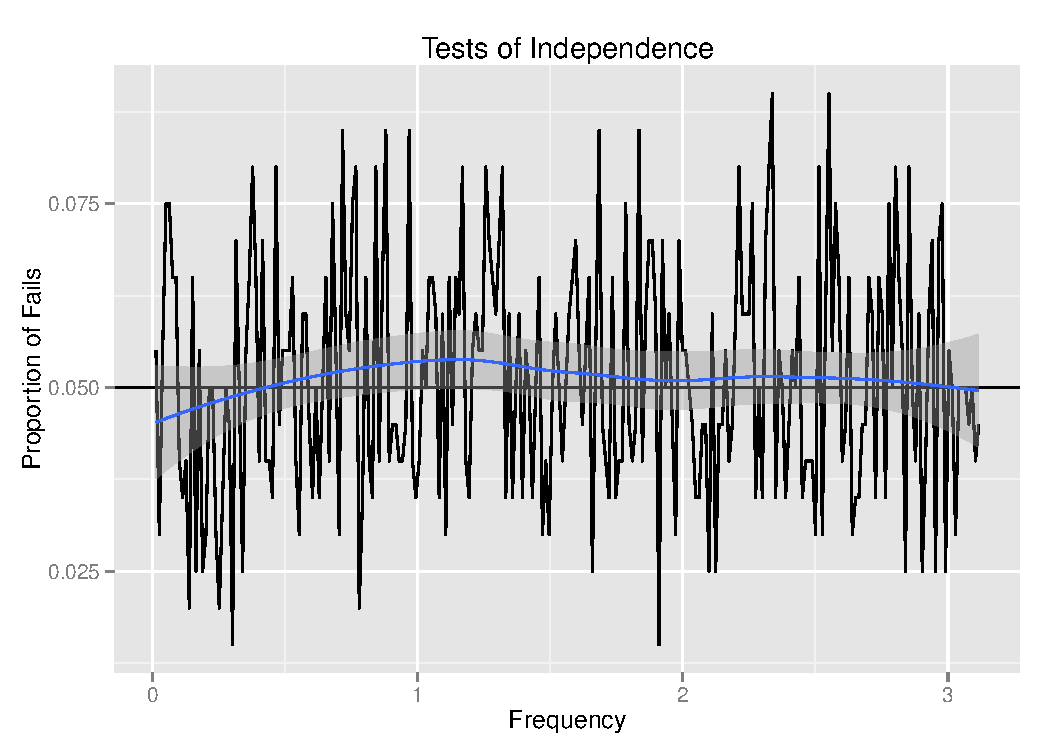
\includegraphics[width=.49\textwidth]{figure/tests-iid1} 
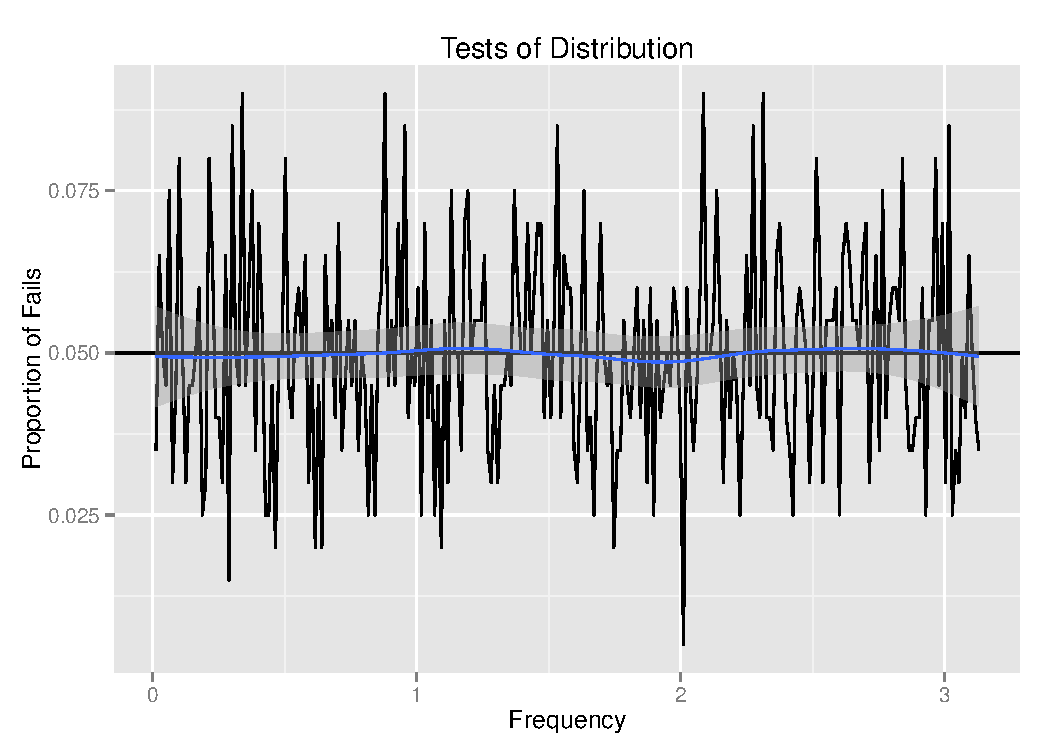
\includegraphics[width=.49\textwidth]{figure/tests-iid2} \caption[Tests of independence and distribution for a Gaussian IID Model]{Tests of independence and distribution for a Gaussian IID Model.\label{fig:tests-iid}}
\end{figure}


\end{knitrout}


\subsubsection{AR(1)}
The first model considered to test the asymptotic assumptions in Results~\ref{res:first} and~\ref{res:lahiri} was an AR(1) model with $\phi = 0.05$. For a timeseries $\{X_t\}$, this model has the form
\begin{align}
x_t = \phi x_{t-1} + \epsilon_t
\end{align}
where $\epsilon_t \sim WN(0, \sigma^2)$. Figure~\ref{fig:inital-ar1} shows that the periodogram for this model shows more structure than that of the IID Gaussian with frequencies closer to 0 showing up as of higher importance than those further from 0. 
\begin{knitrout}
\definecolor{shadecolor}{rgb}{0.969, 0.969, 0.969}\color{fgcolor}\begin{figure}[H]

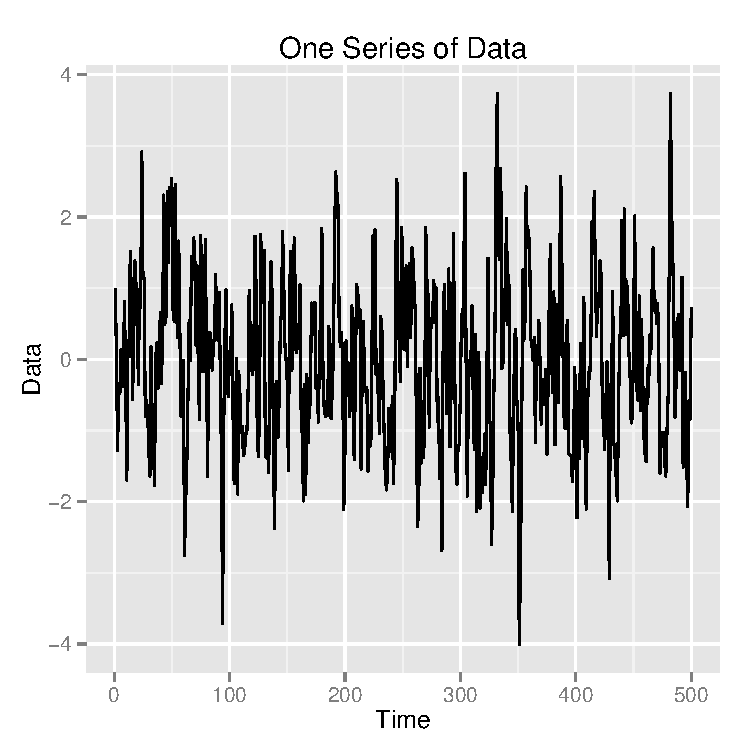
\includegraphics[width=.33\textwidth]{figure/inital-ar11} 
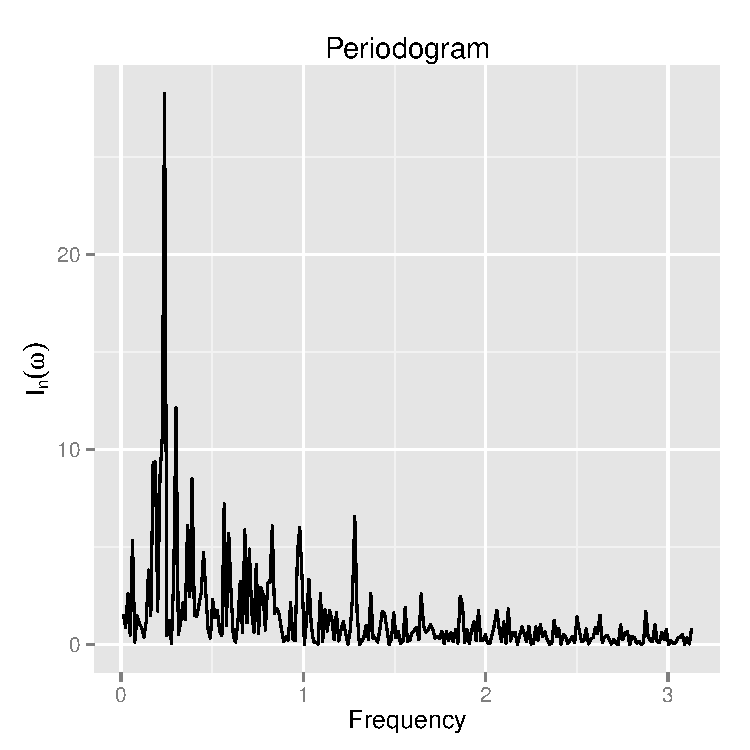
\includegraphics[width=.33\textwidth]{figure/inital-ar12} 
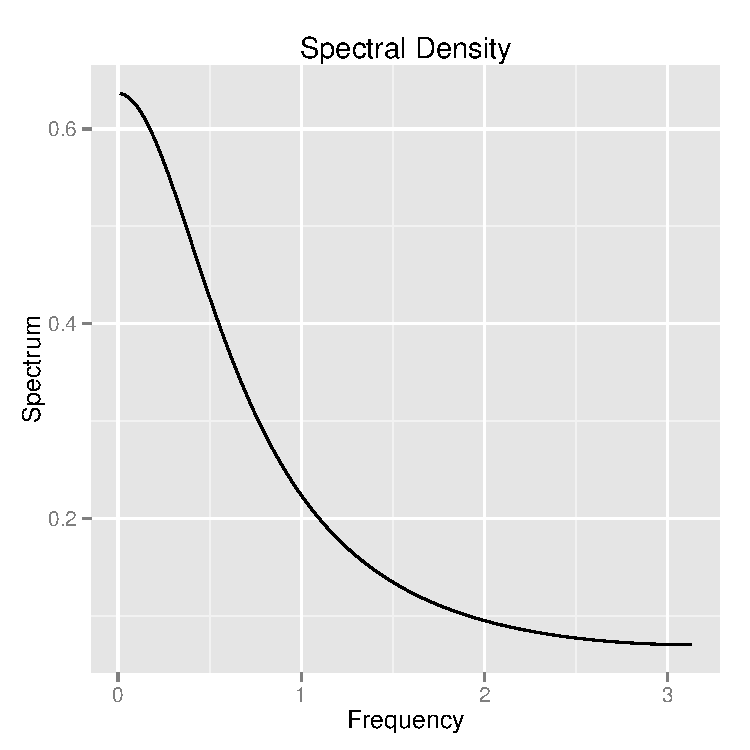
\includegraphics[width=.33\textwidth]{figure/inital-ar13} \caption[One draw, periodogram, and spectral density of an AR(1) model]{One draw, periodogram, and spectral density of an AR(1) model.\label{fig:inital-ar1}}
\end{figure}


\end{knitrout}


The tests of exponential distributions and pairwise independence also gave rejection results consistent with the Type I error rate. Therefore, there was no indication that Result~\ref{res:first} does not hold at the Fourier frequencies for an AR(1) model with $\phi=0.5$. This was not entirely surprising as an AR(1) model has only slightly more structure than a white noise model as it represents dependence between neighboring time points only.
\begin{knitrout}
\definecolor{shadecolor}{rgb}{0.969, 0.969, 0.969}\color{fgcolor}\begin{figure}[H]

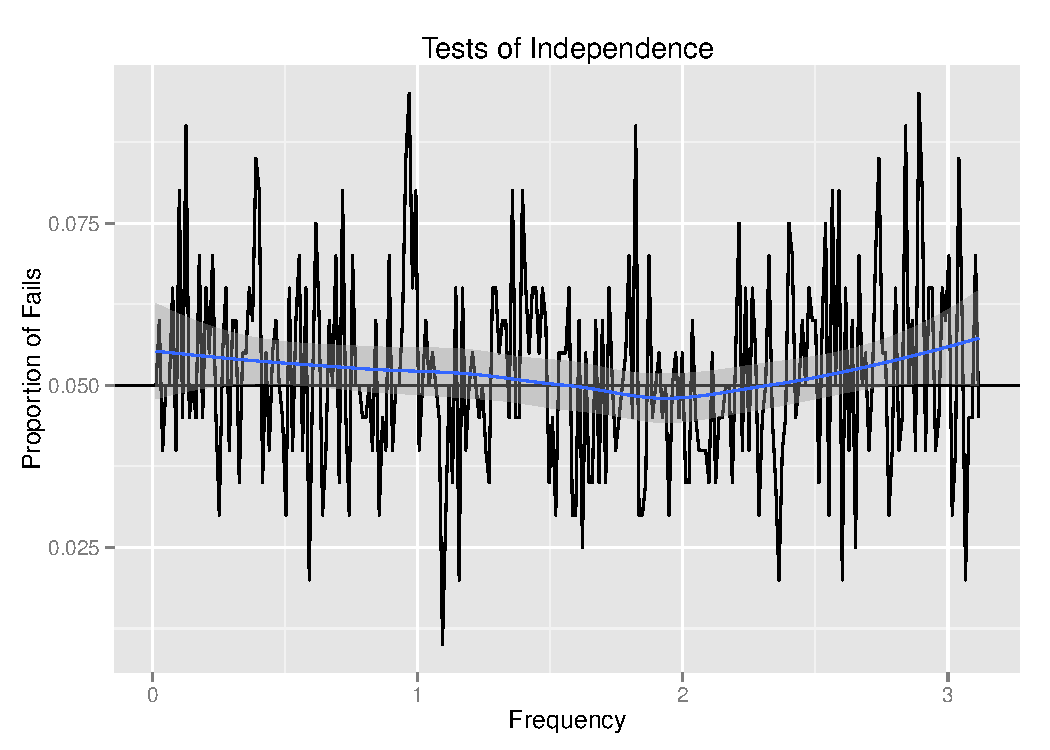
\includegraphics[width=.49\textwidth]{figure/tests-ar11} 
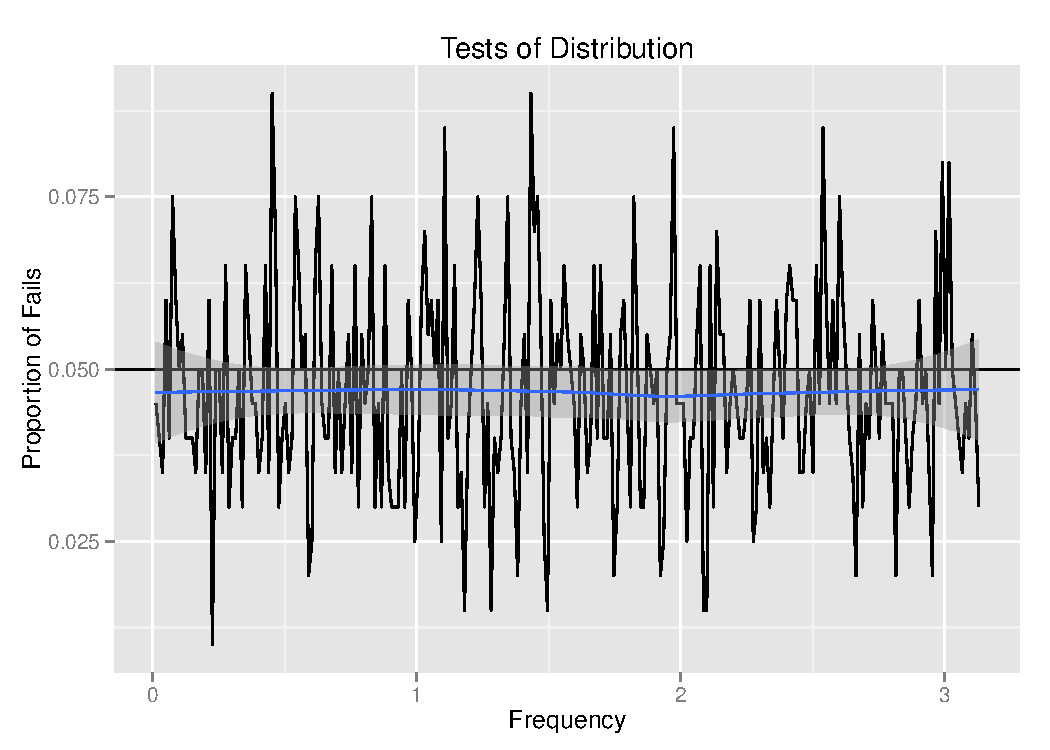
\includegraphics[width=.49\textwidth]{figure/tests-ar12} \caption[Tests of independence and distribution for an AR(1) model]{Tests of independence and distribution for an AR(1) model.\label{fig:tests-ar1}}
\end{figure}


\end{knitrout}


\subsubsection{AR(4)}
To experiment with a timeseries with a slightly more long-term structure, we implemented an AR(4) model with $\boldsymbol{\phi} = [0.08, 0.33, 0.1, 0.45]$. The estimated periodogram, for simulated timeseries following this model, is dominated by frequencies very close to 0, Figure~\ref{fig:inital-ar4}. 
\begin{knitrout}
\definecolor{shadecolor}{rgb}{0.969, 0.969, 0.969}\color{fgcolor}\begin{figure}[H]

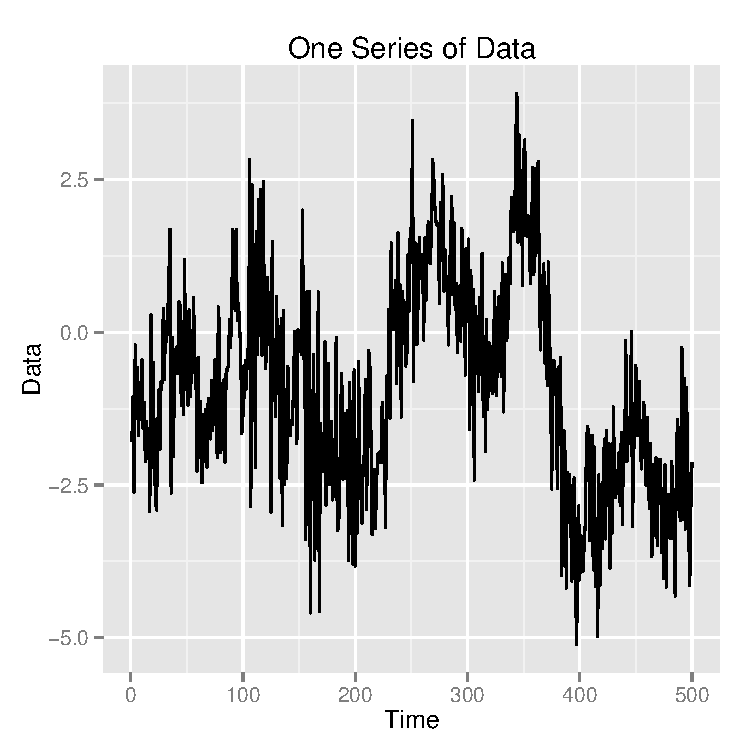
\includegraphics[width=.33\textwidth]{figure/inital-ar41} 
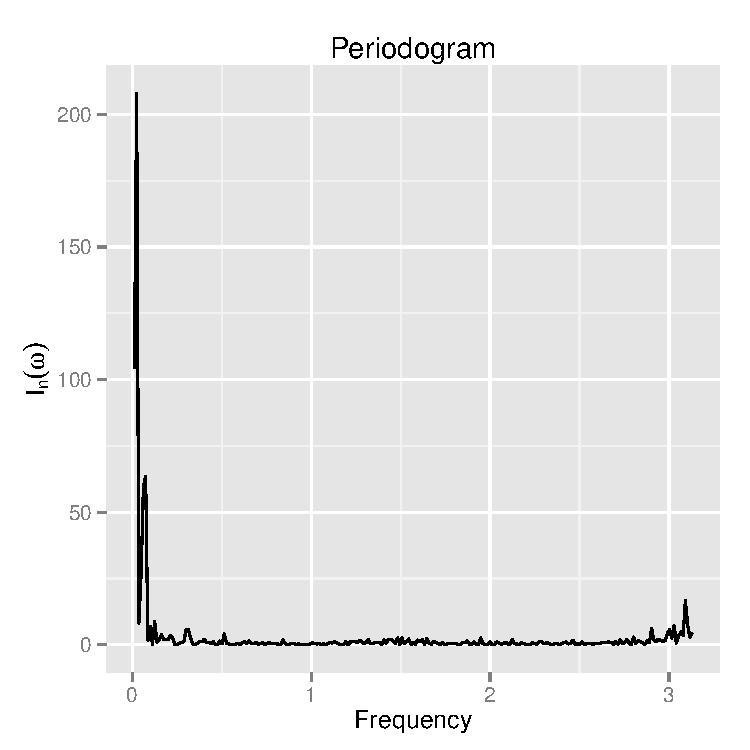
\includegraphics[width=.33\textwidth]{figure/inital-ar42} 
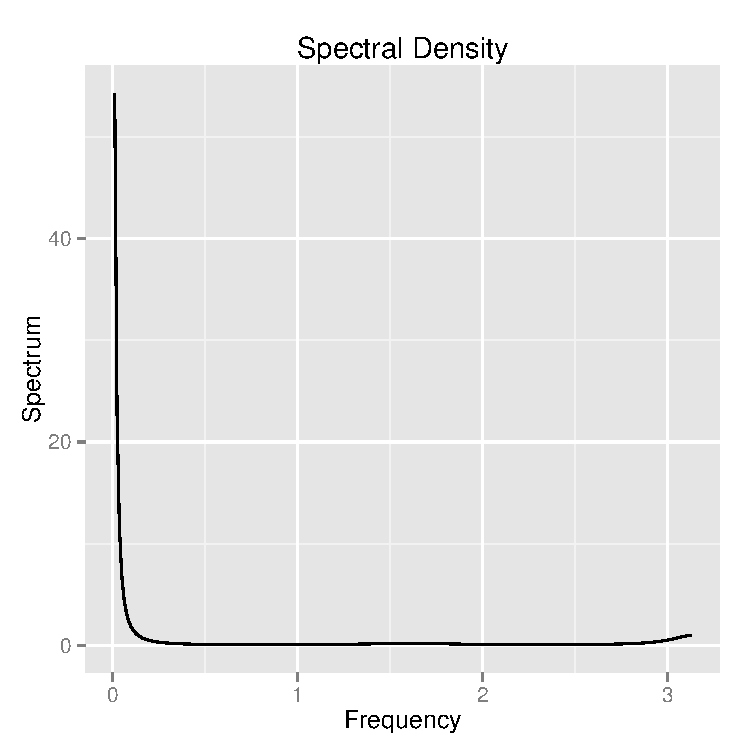
\includegraphics[width=.33\textwidth]{figure/inital-ar43} \caption[One draw, periodogram, and spectral density of an AR(4) model]{One draw, periodogram, and spectral density of an AR(4) model.\label{fig:inital-ar4}}
\end{figure}


\end{knitrout}


Unlike the IID Gaussian and AR(1) models, this AR(4) model does not have rejection rates all close to $\alpha$ for the independence and exponential tests at neighboring Fourier frequencies. At frequencies closer to 0, the pairwise independence tests fail at rates consistently higher than $\alpha$ and likewise, especially for frequencies less than 1, the periodogram ordinates should not be considered to be asymptotically exponentially distributed. Sparcifying the Fourier frequencies closer to 0 will not change that the periodograms at these frequencies are asymptotically exponential. However, we explore if sparcifying the frequencies closer to 0 will satisfy Result~\ref{res:lahiri} in Section~\ref{sec:sparce}.

\begin{knitrout}
\definecolor{shadecolor}{rgb}{0.969, 0.969, 0.969}\color{fgcolor}\begin{figure}[H]

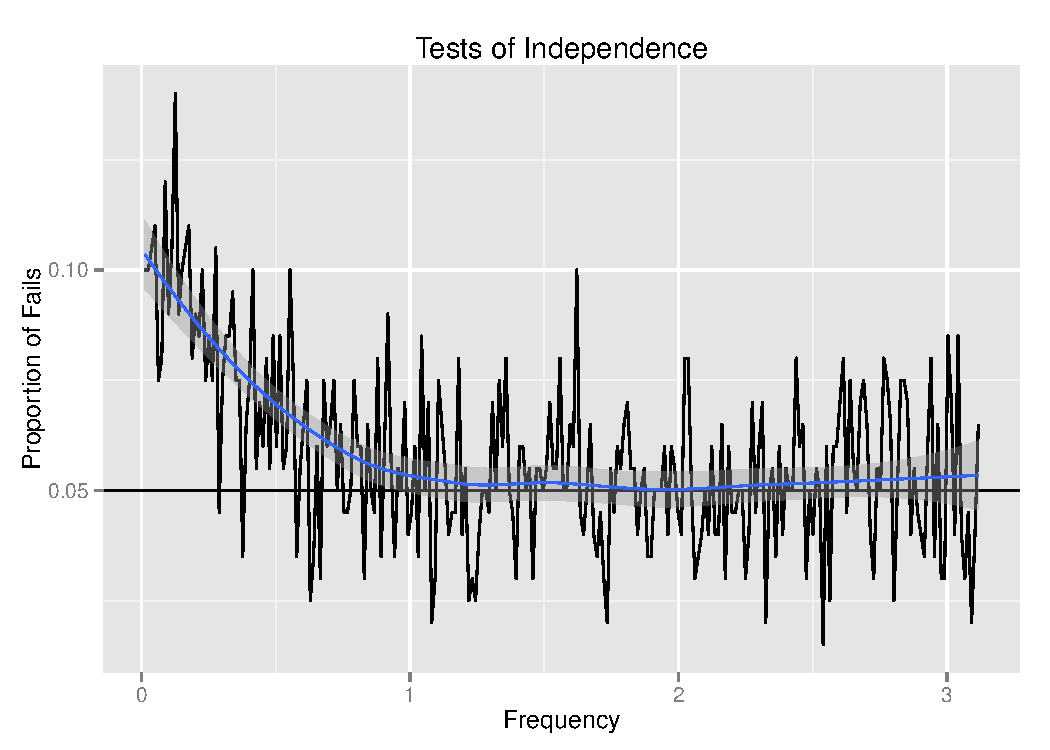
\includegraphics[width=.49\textwidth]{figure/tests-ar41} 
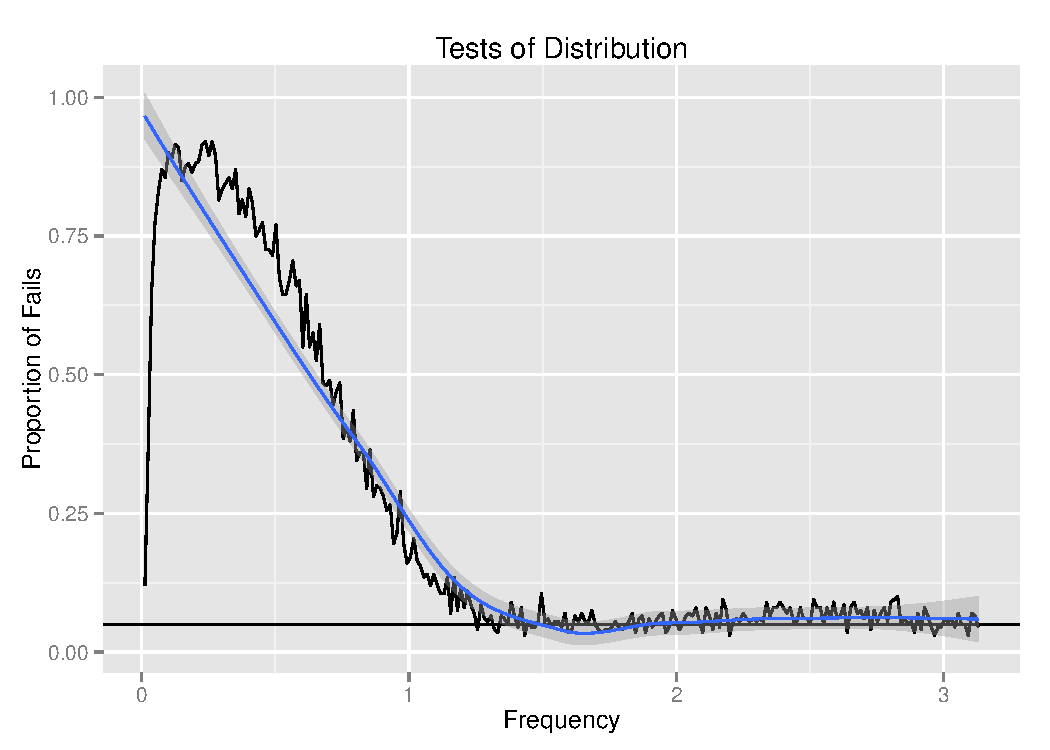
\includegraphics[width=.49\textwidth]{figure/tests-ar42} \caption[Tests of independence and distribution for an AR(4) model]{Tests of independence and distribution for an AR(4) model.\label{fig:tests-ar4}}
\end{figure}


\end{knitrout}


\subsubsection{MA(1)}
\begin{knitrout}
\definecolor{shadecolor}{rgb}{0.969, 0.969, 0.969}\color{fgcolor}\begin{figure}[H]

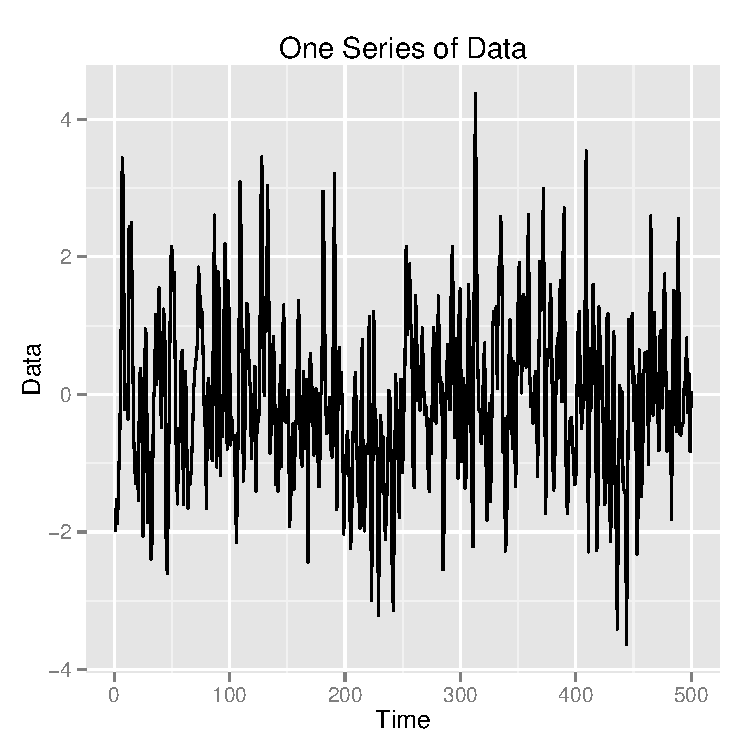
\includegraphics[width=.33\textwidth]{figure/inital-ma11} 
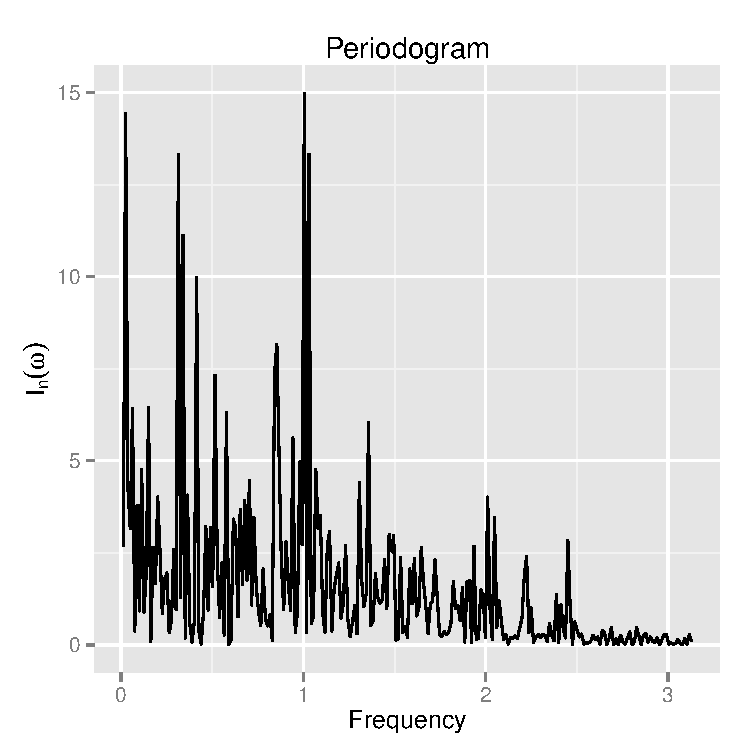
\includegraphics[width=.33\textwidth]{figure/inital-ma12} 
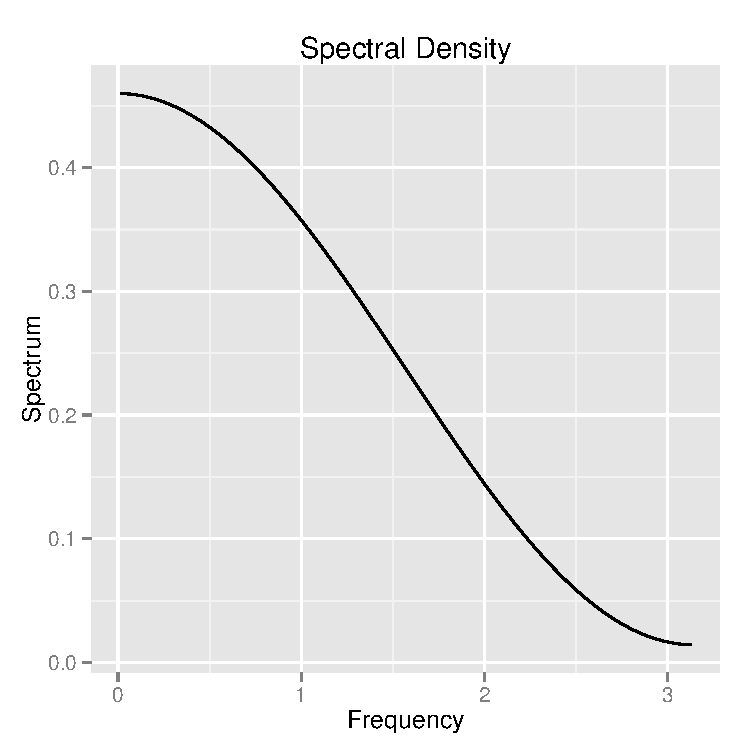
\includegraphics[width=.33\textwidth]{figure/inital-ma13} \caption[One draw, periodogram, and spectral density of an MA(1) model]{One draw, periodogram, and spectral density of an MA(1) model.\label{fig:inital-ma1}}
\end{figure}


\end{knitrout}


\begin{knitrout}
\definecolor{shadecolor}{rgb}{0.969, 0.969, 0.969}\color{fgcolor}\begin{figure}[H]

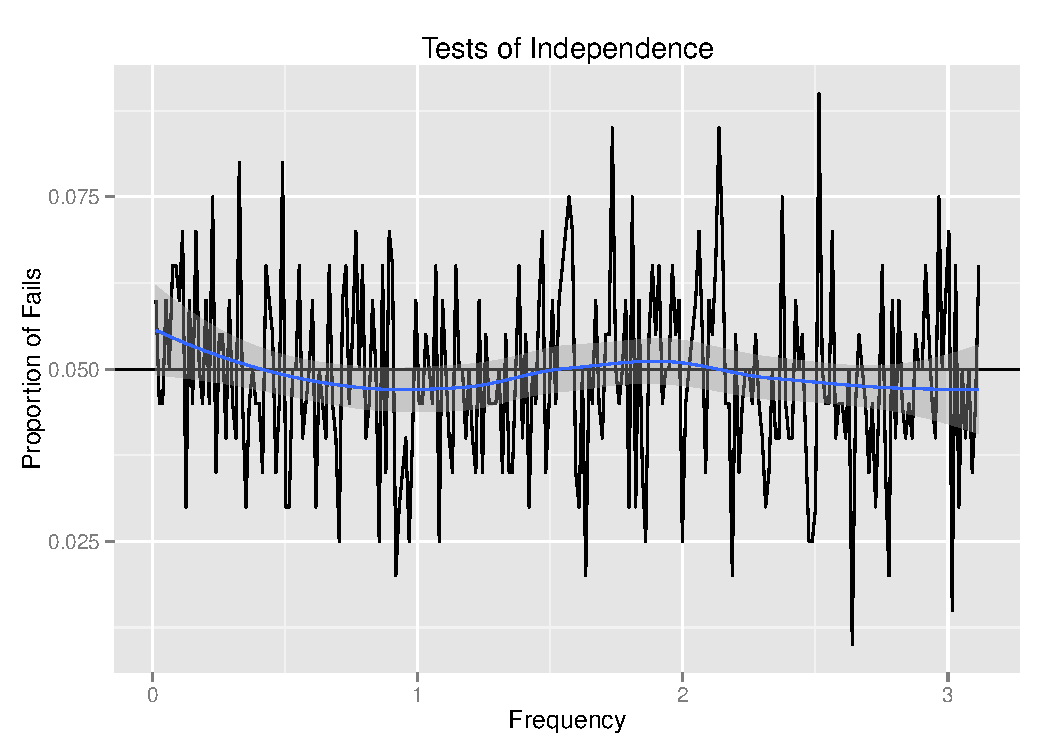
\includegraphics[width=.49\textwidth]{figure/tests-ma11} 
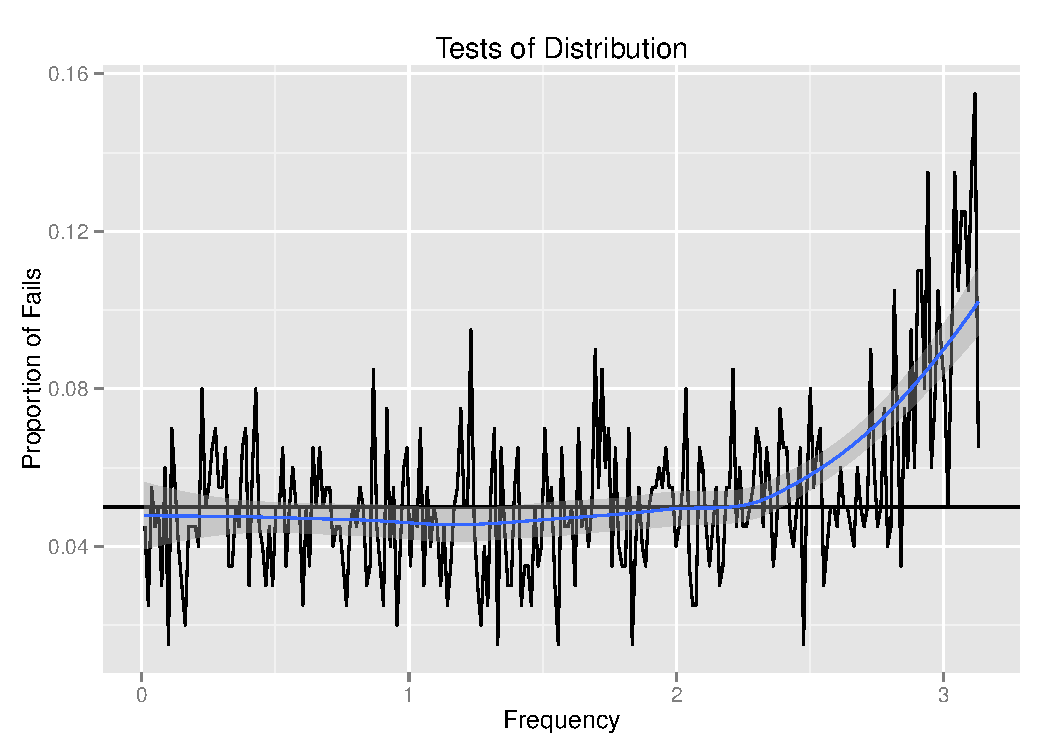
\includegraphics[width=.49\textwidth]{figure/tests-ma12} \caption[Tests of independence and distribution for an MA(1) model]{Tests of independence and distribution for an MA(1) model.\label{fig:tests-ma1}}
\end{figure}


\end{knitrout}


% \subsubsection{MA(2)}
% <<inital-ma2, echo=FALSE, fig.show='hold', fig.width=5, fig.height=5, out.width='.33\\textwidth', fig.cap='One draw, periodogram, and spectral density of an MA(2) model.', fig.pos='H'>>=
% g_draws.ma2
% g_perio.ma2
% g_spec.ma2
% @
% 
% <<tests-ma2, echo=FALSE, fig.show='hold', fig.width=7, fig.height=5, out.width='.49\\textwidth', fig.cap='Tests of independence and distribution for an MA(2) model.', fig.pos='H'>>=
% g_ind.ma2
% g_exp.ma2
% @
% 
\subsubsection{ARMA(4,1)}
\begin{knitrout}
\definecolor{shadecolor}{rgb}{0.969, 0.969, 0.969}\color{fgcolor}\begin{figure}[H]

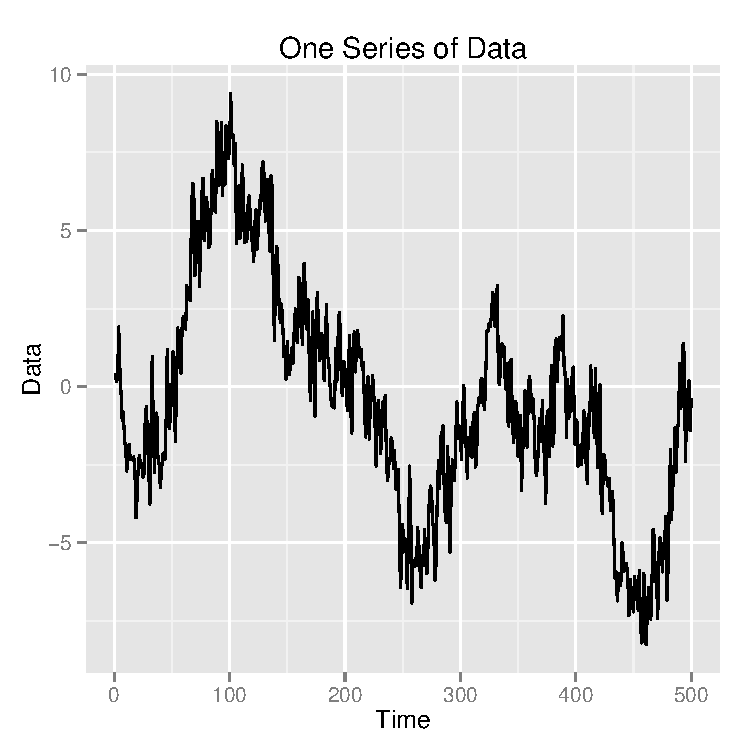
\includegraphics[width=.33\textwidth]{figure/inital-arma411} 
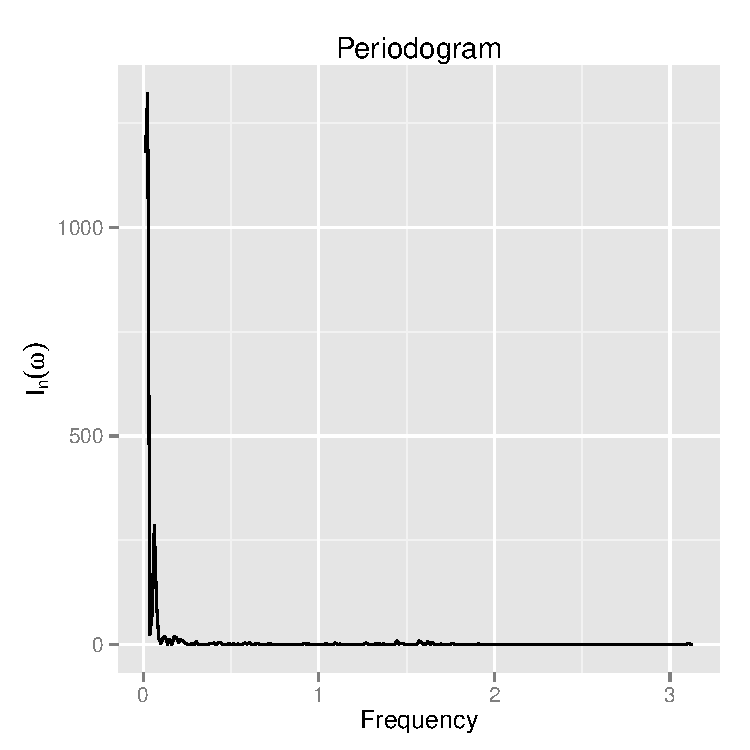
\includegraphics[width=.33\textwidth]{figure/inital-arma412} 
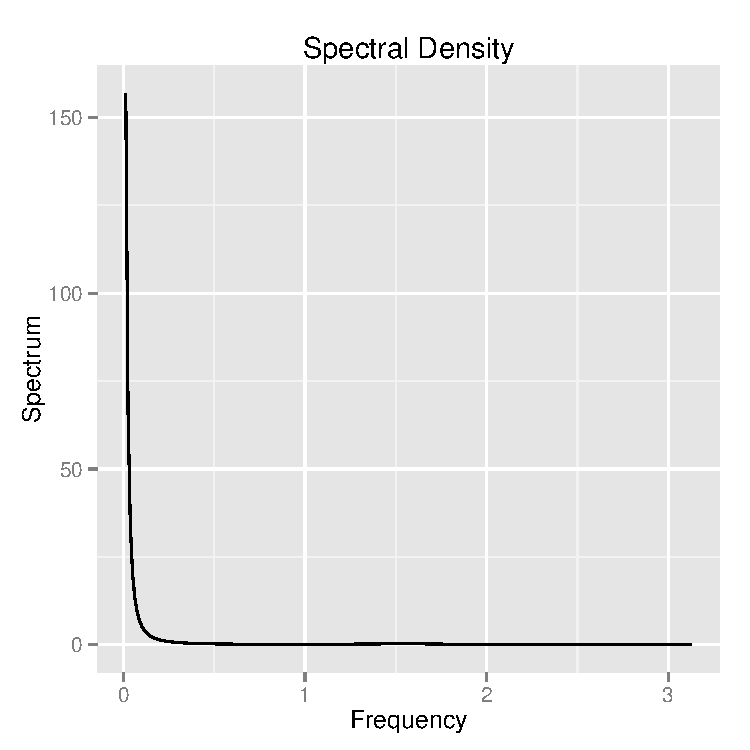
\includegraphics[width=.33\textwidth]{figure/inital-arma413} \caption[One draw, periodogram, and spectral density of an ARMA(4,1) model]{One draw, periodogram, and spectral density of an ARMA(4,1) model.\label{fig:inital-arma41}}
\end{figure}


\end{knitrout}


\begin{knitrout}
\definecolor{shadecolor}{rgb}{0.969, 0.969, 0.969}\color{fgcolor}\begin{figure}[H]

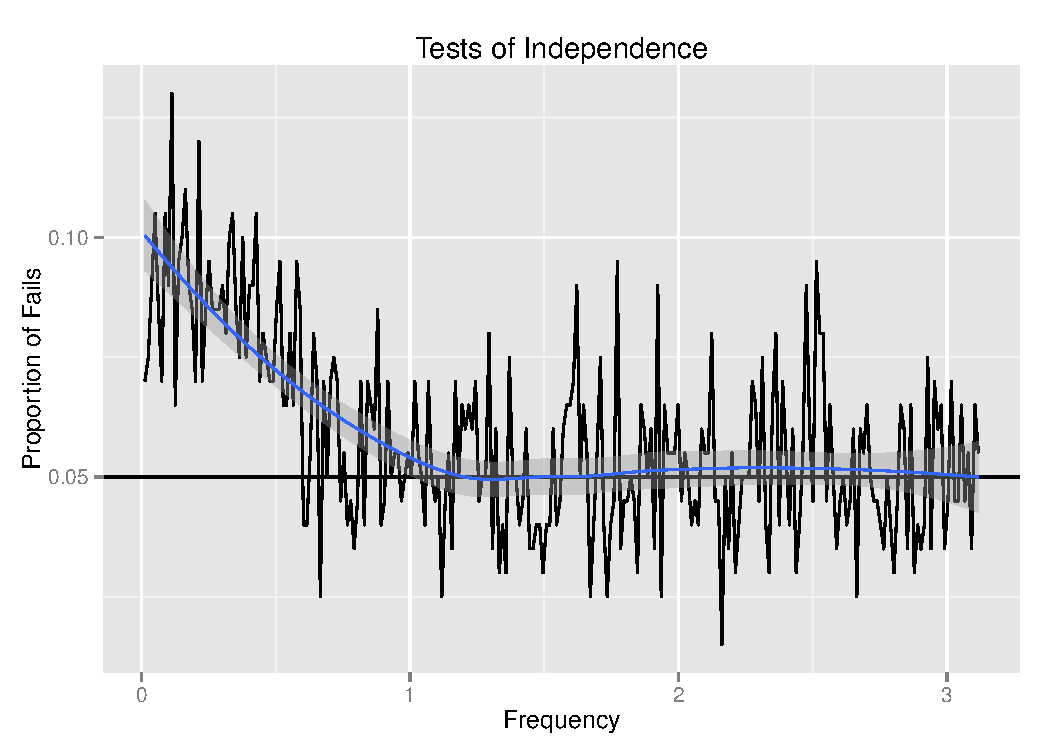
\includegraphics[width=.49\textwidth]{figure/tests-arma411} 
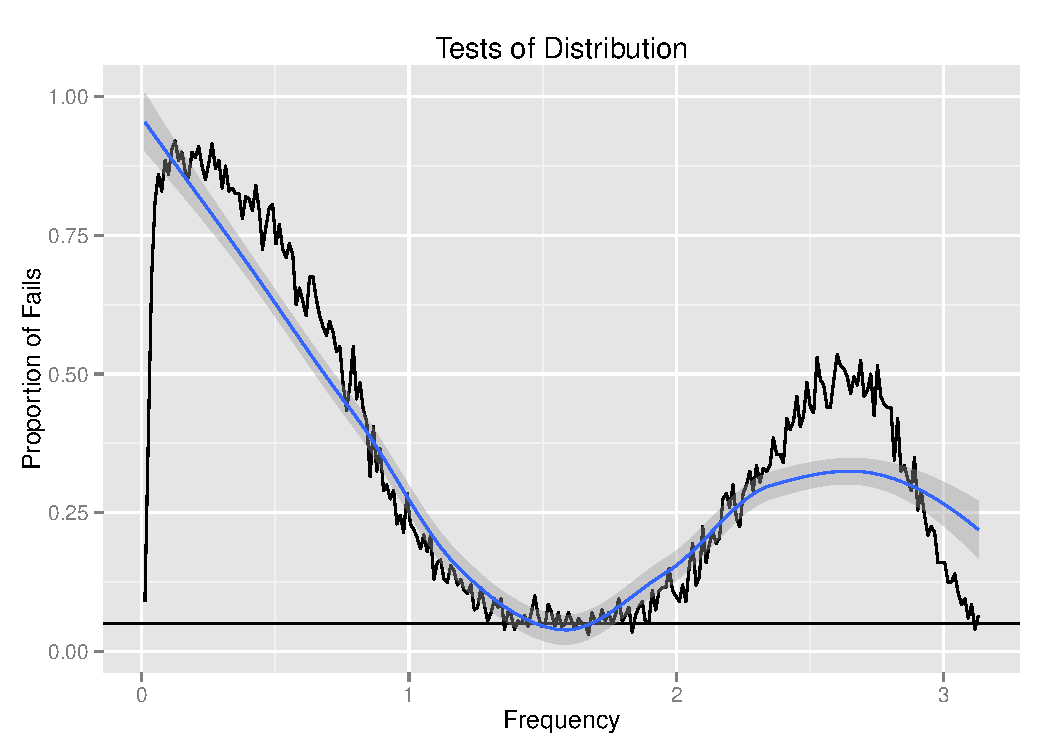
\includegraphics[width=.49\textwidth]{figure/tests-arma412} \caption[Tests of independence and distribution for an ARMA(4,1) model]{Tests of independence and distribution for an ARMA(4,1) model.\label{fig:tests-arma41}}
\end{figure}


\end{knitrout}


% \subsubsection{ARMA(4,2)}
% <<inital-arma42, echo=FALSE, fig.show='hold', fig.width=5, fig.height=5, out.width='.33\\textwidth', fig.cap='One draw, periodogram, and spectral density of an ARMA(4,2) model.', fig.pos='H'>>=
% g_draws.arma42
% g_perio.arma42
% g_spec.arma42
% @
% 
% <<tests-arma42, echo=FALSE, fig.show='hold', fig.width=7, fig.height=5, out.width='.49\\textwidth', fig.cap='Tests of independence and distribution for an ARMA(4,2) model.', fig.pos='H'>>=
% g_ind.arma42
% g_exp.arma42
% @

\subsection{Sparcify Frequencies for AR(4)} \label{sec:sparce}


\section{Discussion}


\mj{
\paragraph{Issues}
\begin{enumerate}
  \item Multiple comparison 
  \item ARMA(4,2), MA(1), MA(2)
  \item Exponential Fails
  \item Usability 
  \begin{itemize}
    \item ARMA useless, Models w/more structure 
    \item spacing depends on model
    \item can never really be used in practice
  \end{itemize}
  \item Computation time
  \item Pairwise independence $\neq$ Joint independence
\end{enumerate}}


\printbibliography

\end{document}
